\documentclass[12pt,a4paper,openright,twoside]{book}
\usepackage[utf8]{inputenc}
\usepackage{disi-thesis}
\usepackage{code-lstlistings}
\usepackage{notes}
\usepackage{shortcuts}
\usepackage{acronym}
\usepackage{placeins}

\school{\unibo}
\programme{Corso di Laurea in Ingegneria e Scienze Informatiche}
\title{Fancy Title}
\author{Candidate Name}
\date{\today}
\subject{Supervisor's course name}
\supervisor{Prof. Supervisor Here}
\cosupervisor{Dott. CoSupervisor 1}
\morecosupervisor{Dott. CoSupervisor 2}
\session{I}
\academicyear{2022-2023}

% Definition of acronyms
\acrodef{IoT}{Internet of Thing}
\acrodef{vm}[VM]{Virtual Machine}


\mainlinespacing{1.241} % line spacing in mainmatter, comment to default (1)

\begin{document}

\frontmatter\frontispiece

\begin{abstract}	
Max 2000 characters, strict.
\end{abstract}

\begin{dedication} % this is optional
Optional. Max a few lines.
\end{dedication}

%----------------------------------------------------------------------------------------
\tableofcontents   
\listoffigures     % (optional) comment if empty
%\lstlistoflistings % (optional) comment if empty
%----------------------------------------------------------------------------------------

\mainmatter

% TODO: rileggere, andare a capo, typos
\chapter{Contesto e obbiettivi del progetto}
% Introduzione al contesto, le necessità e l'ambiente.
Il progetto si inserisce all'interno di una serie di studi di fattibilità volti all'implementazione di servizi informatici sull'infrastruttura virtualizzata dell'Istituto Nazionale di Geofisica e Vulcanologia (INGV).
L'esigenza di disporre di un'infrastruttura interna nasce dalla volontà di ridurre i costi associati all'adozione di servizi cloud commerciali, e dalla necessità di avere un ambiente personalizzato, sicuro e pienamente amministrabile,
in cui gestire in modo autonomo le risorse destinate agli utenti.
% Spiegazione della VDC.
Il risultato di questo approccio è la creazione di un Virtual Data Center (VDC): un ambiente virtualizzato in cui ogni tenant ha la possibilità di definire e gestire autonomamente risorse come macchine virtuali, reti, VPN, e gateway di accesso.
Il tutto avviene senza la necessità di interagire direttamente con l'infrastruttura fisica sottostante, la cui gestione è demandata al personale IT.
Ciò permette agli utenti di operare in un ambiente flessibile, mantenendo comunque un alto grado di controllo e isolamento.

% Escursus su NEREIDE
Il progetto Nereide (NEw REsearch Infrastructure Datacenter for EMSO), sviluppato da INGV presso la sede di Portopalo di Capo Passero e parte integrante della rete EMSO-ERIC, rappresenta un esempio concreto di questa visione.
Esso fornisce VDC basati su tecnologie OpenStack e Ceph, offrendo risorse computazionali e di storage scalabili e sicure.
Nereide è progettato per accelerare i flussi di lavoro della data science, in particolare in ambito marino, sostenendo i principi FAIR (Findable, Accessible, Interoperable, Reusable) e l'integrazione con ecosistemi federati come Blue-Cloud e il Digital Twin of the Ocean\cite{cacciaguerra2024vdc}.

% Introduzione alla necessità di installare servizi da zero. 
Il problema introdotto dalla creazione dei VDC è la necessità di installare e configurare da zero i servizi che le piattaforme cloud offrono come \textit{managed} come Slurm, JupyterLab e Kubernetes. 
Da qui l'obiettivo specifico di questo progetto, che è la realizzazione di script Infrastructure-as-Code (IaC) che permettano la creazione automatizzata di cluster Kubernetes all'interno dei VDC di Nereide.
Questo approccio consente la definizione e il deploy di ambienti complessi tramite codice versionato e ripetibile, riducendo drasticamente il carico operativo per gli utenti finali e favorendo la riproducibilità della ricerca.

% Riflessione sull'uso di cluster su infrastrutture virtualizzate.
Una riflessione importante riguarda il posizionamento di cluster come Kubernetes o Slurm su infrastrutture virtualizzate anziché fisiche.
Sebbene questa scelta possa sembrare controintuitiva per chi cerca prestazioni ottimali, in questo contesto essa rappresenta una soluzione efficace e pragmatica.
Le infrastrutture virtuali offrono vantaggi notevoli in termini di facilità di gestione, rapidità di provisioning, condivisione tra progetti, e prototipazione agile.
Gli utenti possono evitare la complessità della configurazione di macchine fisiche e accedere rapidamente a un ambiente operativo, riducendo il tempo necessario per iniziare la formazione o la sperimentazione.
Certo, esistono svantaggi — come una ridotta efficienza rispetto al bare-metal — ma questi sono ampiamente compensati dalla flessibilità e dalla capacità di scalare e replicare ambienti in modo rapido e controllato.
In ambito didattico e nelle prime fasi della ricerca, questo compromesso si dimostra vincente: permette ai gruppi di lavoro di operare in autonomia e accelerare il ciclo di vita delle idee, senza dipendere da strutture
esterne o da lunghi processi di approvazione per l'uso di risorse.

% Conclusione
In definitiva, i VDC e l'approccio IaC si rivelano strumenti abilitanti fondamentali per la nuova generazione di ricerca scientifica aperta, distribuita e collaborativa.
Questo progetto si propone di contribuire a questa evoluzione, offrendo soluzioni pratiche per l'automazione e la standardizzazione di ambienti di calcolo avanzati all'interno della piattaforma Nereide.

% Struttura della tesi
% TODO
\chapter{Architettura e componenti utilizzati}
\section{OpenStack}
OpenStack è una piattaforma open-source per la gestione delle infrastrutture cloud. Nell'contesto dell'INGV è stata adottata come piattaforma per la creazione di
macchine virtuali permettendo di dividere le risorse tra diversi gruppi di utenti (detti \textit{tenant}) che possono essere i gruppi di ricerca.
Questa piattaforma è particolarmente flessibile perché, essendo divisa in componenti, permette di scegliere quali utilizzare e come configurarli. Essa può essere
una scelta valida per le imprese o istituzioni che non vogliono dipendere da fornitori di servizi esterni o hanno bisogno di soluzioni personalizzate.
Vediamo elencati ora alcuni dei principali componenti di OpenStack\cite{amslaurea29330}:
%
% TODO: integrare la spiegazione dei componenti, rileggere, andare a capo, typos
%
\begin{itemize}
    \item \textbf{Nova}: è il servizio che gestisce il \textit{provisioning} delle macchine virtuali e fisiche. 
    \item \textbf{Neutron}: gestisce tutti gli aspetti della rete, permettendo la comunicazione tra risorse e componenti di OpenStack. 
    \item \textbf{Cinder}: espone l'API per la gestione dello storage a blocchi, fornendo agli utenti ed alle macchine i volumi necessari.
    \item \textbf{Glance}: mantiene le immagini e metadati che l'utente utilizza in altri servizi. 
    \item \textbf{Keystone}: fornisce autenticazione per l'intera piattaforma. Gestisce utenti, ruoli, progetti e policy di accesso.
    \item \textbf{Horizon}: l'interfaccia web che permette agli utenti di interagire con OpenStack attraverso un browser. Fornisce un'interfaccia grafica per la gestione delle risorse.
\end{itemize}
\begin{figure}
    \centering
    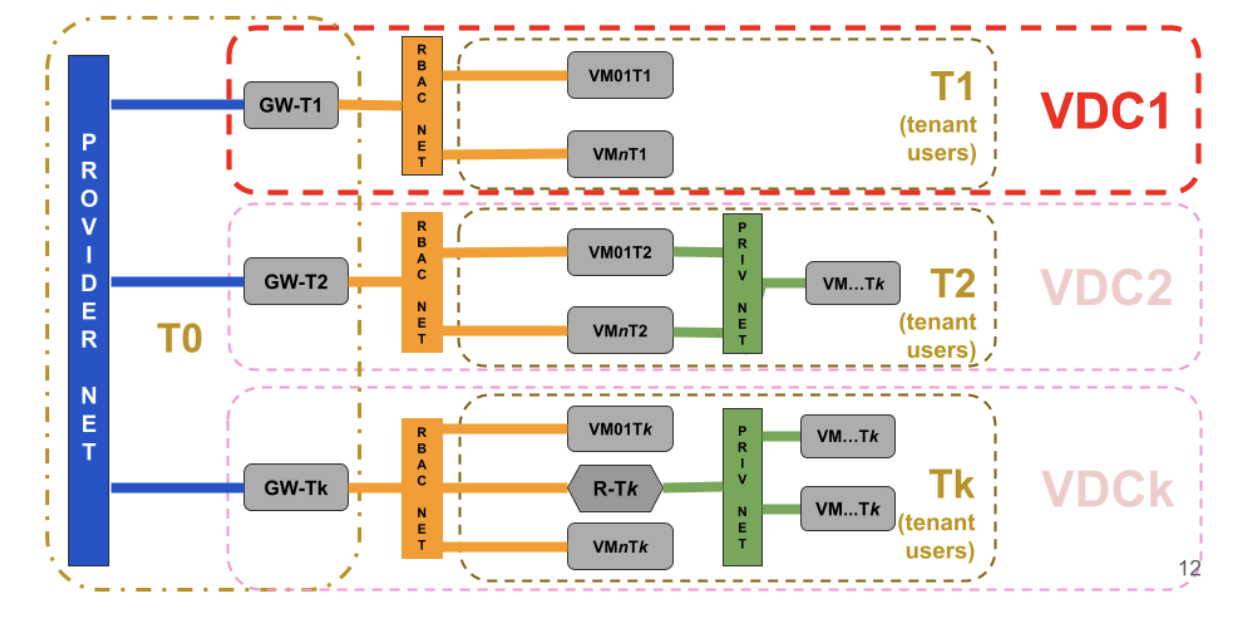
\includegraphics[width=0.6\textwidth]{figures/vdc-diagram.png}
    \caption{Schema di un Virtual Data Center}
    \label{fig:vdc}
\end{figure}
\section{Cloud-Init}
%
% TODO: rileggere, andare a capo, typos
%
Una tecnologia di \textit{Infrastructure-as-Code} (IaC) con cui le istanze vengono configurate automaticamente al loro avvio installando pacchetti, scrivendo file di configurazione e inviando comandi alla shell. \\
IaC è un approccio che automatizza la creazione e gestione dei componenti dell'infrastruttura. Favorisce la standardizzazione ed il versioning velocizzando notevolmente il lavoro degli sviluppatori.
Questo componente è già nativo in OpenStack e quindi rende lo sviluppo veloce soprattutto quando si è in fasi in cui sono necessari diversi riavii. Potrebbe non essere la soluzione giusta in un contesto di produzione infatti vi sono applicativi più completi per l'automazione 
del deployment e l'orchestrazione di un cluster:
\begin{itemize}
    \item \textbf{Heat}: il servizio integrato della suite OpenStack per orchestrare tramite template, che in questo caso non era disponibile.
    \item \textbf{Warewulf}: una piattaforma creata appositamente per il automatizzare il provisioning di cluster HPC dotato di gestione delle immagini e creazione automatica dei nodi. Molto più fluido rispetto a Heat ma non adatto per questo stato del progetto anche perché richiede una configurazione più importante delle macchine virtuali (N.B.: WareWulf esegue il provisioning mentre Heat, Ansible e Cloud-Init eseguono la configurazione della macchina quindi W.W. andrebbe utilizzato assieme a qualche altro tool di configurazione).
    \item \textbf{Ansible}: un'altra valida alternativa a Cloud-Init che permette molta più libertà ed anche la possibilità di un mantenimento continuo delle istanze. A sua volta è più complicato da configurare e richiede un ulteriore nodo master per inviare i moduli ai nodi che controlla.
\end{itemize}
%
\section{Kubernetes}
\label{sec:kube}
%
% TODO: rileggere, andare a capo, typos, spiegazione componenti
%
Kubernetes è un sistema open-source per il deployment e lo scaling di applicazioni containerizzate. 
Lavorando a livello dei container fornisce diversi tool come scaling e load balancing ma lascia agli utenti l'integrazione di logging, monitoraggio e scelta dei componenti da utilizzare.
Ciò apre ad una particolare flessibilità e possibilità di integrazione con parecchie piattaforme cloud, infatti Kubernetes è fornito come servizio \textit{managed} (\textit{Platfrom-as-a-Service}) dai principali fornitori cloud tra cui: Azure Kubernetes Service (AKS), Google Kubernetes Engine (GKE), Oracle Kubernetes Engine (OKE).
Con l'avvento dei microservizi è diventata una delle principali piattaforme per l'implementazione di applicazioni scalabili. 
\subsection{Principali componenti di Kubernetes}
Le applicazioni containerizzate sono dispiegate su componenti detti Pods, questi ultimi sono caricati su uno o più nodi del cluster che possono essere macchine fisiche o virtuali. In ogni nodo sono installati tutti i componenti necessari per controllare i pods e tutti i nodi sono controllati dal nodo master che contiene il layer di gestione del ciclo di vita dei pods.\\
I principali componenti sono quindi:
\begin{itemize}
    \item {
        Nodi: macchine virtuali o fisiche dotate di tutti i componenti per la gestione dei containers. Ogni nodo contiene una container runtime (come CRI o \texttt{containerd}), \texttt{kubelet} (l'agente che gestisce localmente i Pods) ed opzionalmente \texttt{kube-proxy} che implementa una parte del networking.
    }
    \item {
        Pods: la più piccola unità che si può dispiegare su Kubernetes. Ciascun pod contiene uno o più container, tipicamente uno oppure due se strettamente legati ed operano sugli stessi files (sidecar).
    }
    \item {
        Services: in Kubernetes le applicazioni sono distribuite ma forniscono tutte lo stesso \textit{servizio} all'utente o al cluster ed un Service è un modo per unire sotto lo stesso endpoint tutte le applicazioni.\\
        Questo componente permette di gestire la natura effimera dei Pods che possono essere creati e distrutti a runtime quindi l'utente farebbe particolare fatica a tenere traccia dei loro indirizzi.\\
        Fa anche da Load Balancer per distribuire il traffico tra i vari Pods.
    }
    \item {
        Ingress: è un servizio di rete che permette di smistare il traffico in base alle regole indicate dall'utente. Questo permette di erogare diversi servizi provenienti da diversi gruppi di Pods dallo stesso endpoint.\\
        È componente molto potente in quanto può fare da Load Balancer e come terminazione SSL/TLS; queste caratteristiche riducono la necessità di load balancer nel cluster e permette comunicazioni più snelle in quanto il protocollo di sicurezza viene terminato prima dell'ingresso dei pacchetti nel cluster.\\
        È sempre necessario un Ingress Controller per applicare le regole di routing, questo può essere scelto dall'utente o viene fornito dal cloud provider come nel caso di AKS, GKE o OKE. 
    }
    \item {
        Autoscaling: HPA ed Autoscalers sono componenti che permettono lo scaling orizzontale (aumentando il numero di Pods) o verticale aumentando il numero di Pods al fine di mantenere entro una certa soglia l'utilizzo delle risorse.\\
        Kubernetes è in grado di comunicare, attraverso plugin come Autoscaler o Karpenter, con i Cloud Providers al fine di eliminare o aggiungere risorse al cluster in base alle necessità ed alle limitazioni. Per esempio potrebbero essere necessari più nodi per i Pod in scheduling oppure rimuovere nodi per abbassare i costi e \textit{consolidare} il cluster.
    }
    \item {
        Storage: la gestione dello storage a lungo e corto termine. Viene fatto per mezzo di diversi componenti come volumi, volumi persistenti o ConfigMaps.
    }
\end{itemize}
\subsection{Container runtime e plugin CNI}
%
% TODO: rileggere, andare a capo, typos
%
Come menzionate in precedenza Kubernetes lascia all'utente la scelta di diversi componenti tra cui quello per gestire i container e quello per la gestione della rete\cite{kubernetes}.
Al fine di eseguire i container Kubernetes ha bisogno di un ambiente di esecuzione che implementi la \textit{Container Runtime Interface} (CRI).
Questa interfaccia permette di astrarre il layer di esecuzione dei container e permette a Kubernetes di essere indipendente dal tipo di container runtime utilizzato. 
Sarà quindi sufficiente che il container runtime implementi la CRI per essere utilizzato da Kubernetes, le più note implementazioni sono:
\begin{itemize}
    \item \textbf{Docker Engine}: utilizza internamente containerd e la sua installazione fornisce anche strumenti in linea di comando per la gestione dei container. 
        È necessario installare anche \texttt{cri-dockerd}, un adattatore che permette a Kubernetes e Docker di comunicare tramite la CRI.
    \item \textbf{containerd}: un gestore di container open-source appositamente sviluppato per il cloud che non necessità di nessun componente aggiuntivo. 
        Questo si interfaccia col sistema operativo per eseguire i container.
    \item \textbf{CRI-O}: un container runtime sviluppato per Kubernetes che implementa la CRI. Utilizza \texttt{runc} (come anche containerd) per eseguire i container ma potrebbe utilizzare
        tutti i runtime che implementano la Open Container Initiative (OCI).
\end{itemize}
Oltre al container runtime Kubernetes ha bisogno di un plugin che gestisca le comunicazioni all'interno del cluster; questo è
necessario per implementare il modello di rete di Kubernetes come l'assegnazione di indirizzi IP ai pod oppure l'implementazione dell'API Service.
Il plugin deve essere conforme con la \textit{Container Network Interface} (CNI) e ne sono disponibili varie distribuzioni, quella scelta per questo progetto è
\textit{Calico}.
%
\chapter{Implementazione}
\section{Provisioning delle macchine}
Le macchine virtuali vengono create tramite l'interfaccia grafica di OpenStack (Horizon). Viene scelto di allocare diverse risorse ai nodi, precisamente: 
\begin{itemize}
    \item Al nodo master vengono allocate più risorse rispetto ai nodi worker perché questo deve eseguire diversi processi per il mantenimento del cluster
        come \texttt{kube-proxy} per la gestione della rete, \texttt{kube-scheluder} per l'assegnazione dei pod ai nodi, \texttt{kube-apiserver} per la API di Kubernetes etc.
    \item Ai nodi worker viene allocata una quantità più moderata di risorse ma comunque sufficiente per eseguire diversi pods. 
\end{itemize}
Chiaramente queste risorse sono relative al carico di lavoro che il cluster deve affrontare, nel caso si attenda un lavoro più intenso o si stia progettando per un ambiente di produzione
si può decidere di avviare le macchine già con più risorse a disposizione.

Inoltre in ambienti di produzione è opportuno distribuire i componenti di controllo del cluster (\textit{control plane}) su più nodi master. In questo caso ciascun nodo master eseguirà un'istanza
di ciascun componente e le API verranno esposte al resto del cluster attraverso un load balancer che bilancerà il carico nei vari nodi master (v. \Cref{fig:kube-ha-topo}). E' indicato distribuire i nodi in diversi datacenter 
(chiamati negli ambienti cloud \textit{availability zones}) per mitigare il rischio di interruzione dei servizi\cite{kubernetes}.
%
\FloatBarrier
\begin{figure}
    \centering
    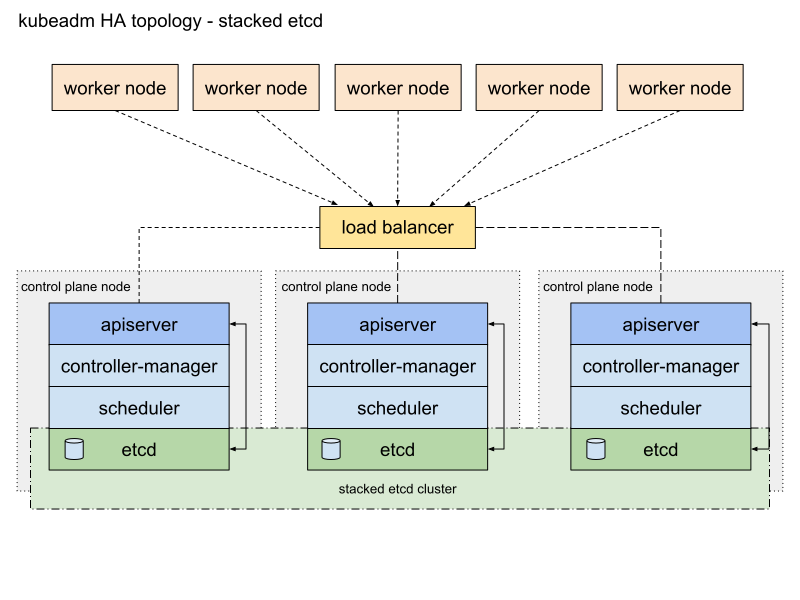
\includegraphics[width=0.8\textwidth]{figures/kube-ha-topo.png}
    \caption{Possibile architettura di una cluster Kubernetes ad alta disponiblità}
    \label{fig:kube-ha-topo}
\end{figure}
%
\section{Configurazione ed installazione dei pacchetti}
Cloud-Init si occupa dell'installazione e configurazione preliminare dei nodi, in particolare:
\begin{itemize}
    \item installa i pacchetti necessari per il funzionamento del cluster: \texttt{containerd}, \texttt{kubeadm}, \texttt{kubectl} e \texttt{kubelet}
    \item l'impostazione di \texttt{Systemd} come cgroup manager per \texttt{containerd} e Kubernetes
    \item l'attivazione di \textit{ip forwading} per permettere ai nodi di scambiare pacchetti tra di loro
    \item l'installazione del plugin CNI \textit{Calico} per la gestione della rete
    \item infine, l'avvio del cluster
\end{itemize}
Un cluster composto da un nodo master e tre nodi worker sarà composto come in figura \ref{fig:kube-cluster}. Ovviamente l'architettura del cluster cambia in base all'ambiente in cui viene disposto.
\begin{figure}[!hbt]
    \centering
    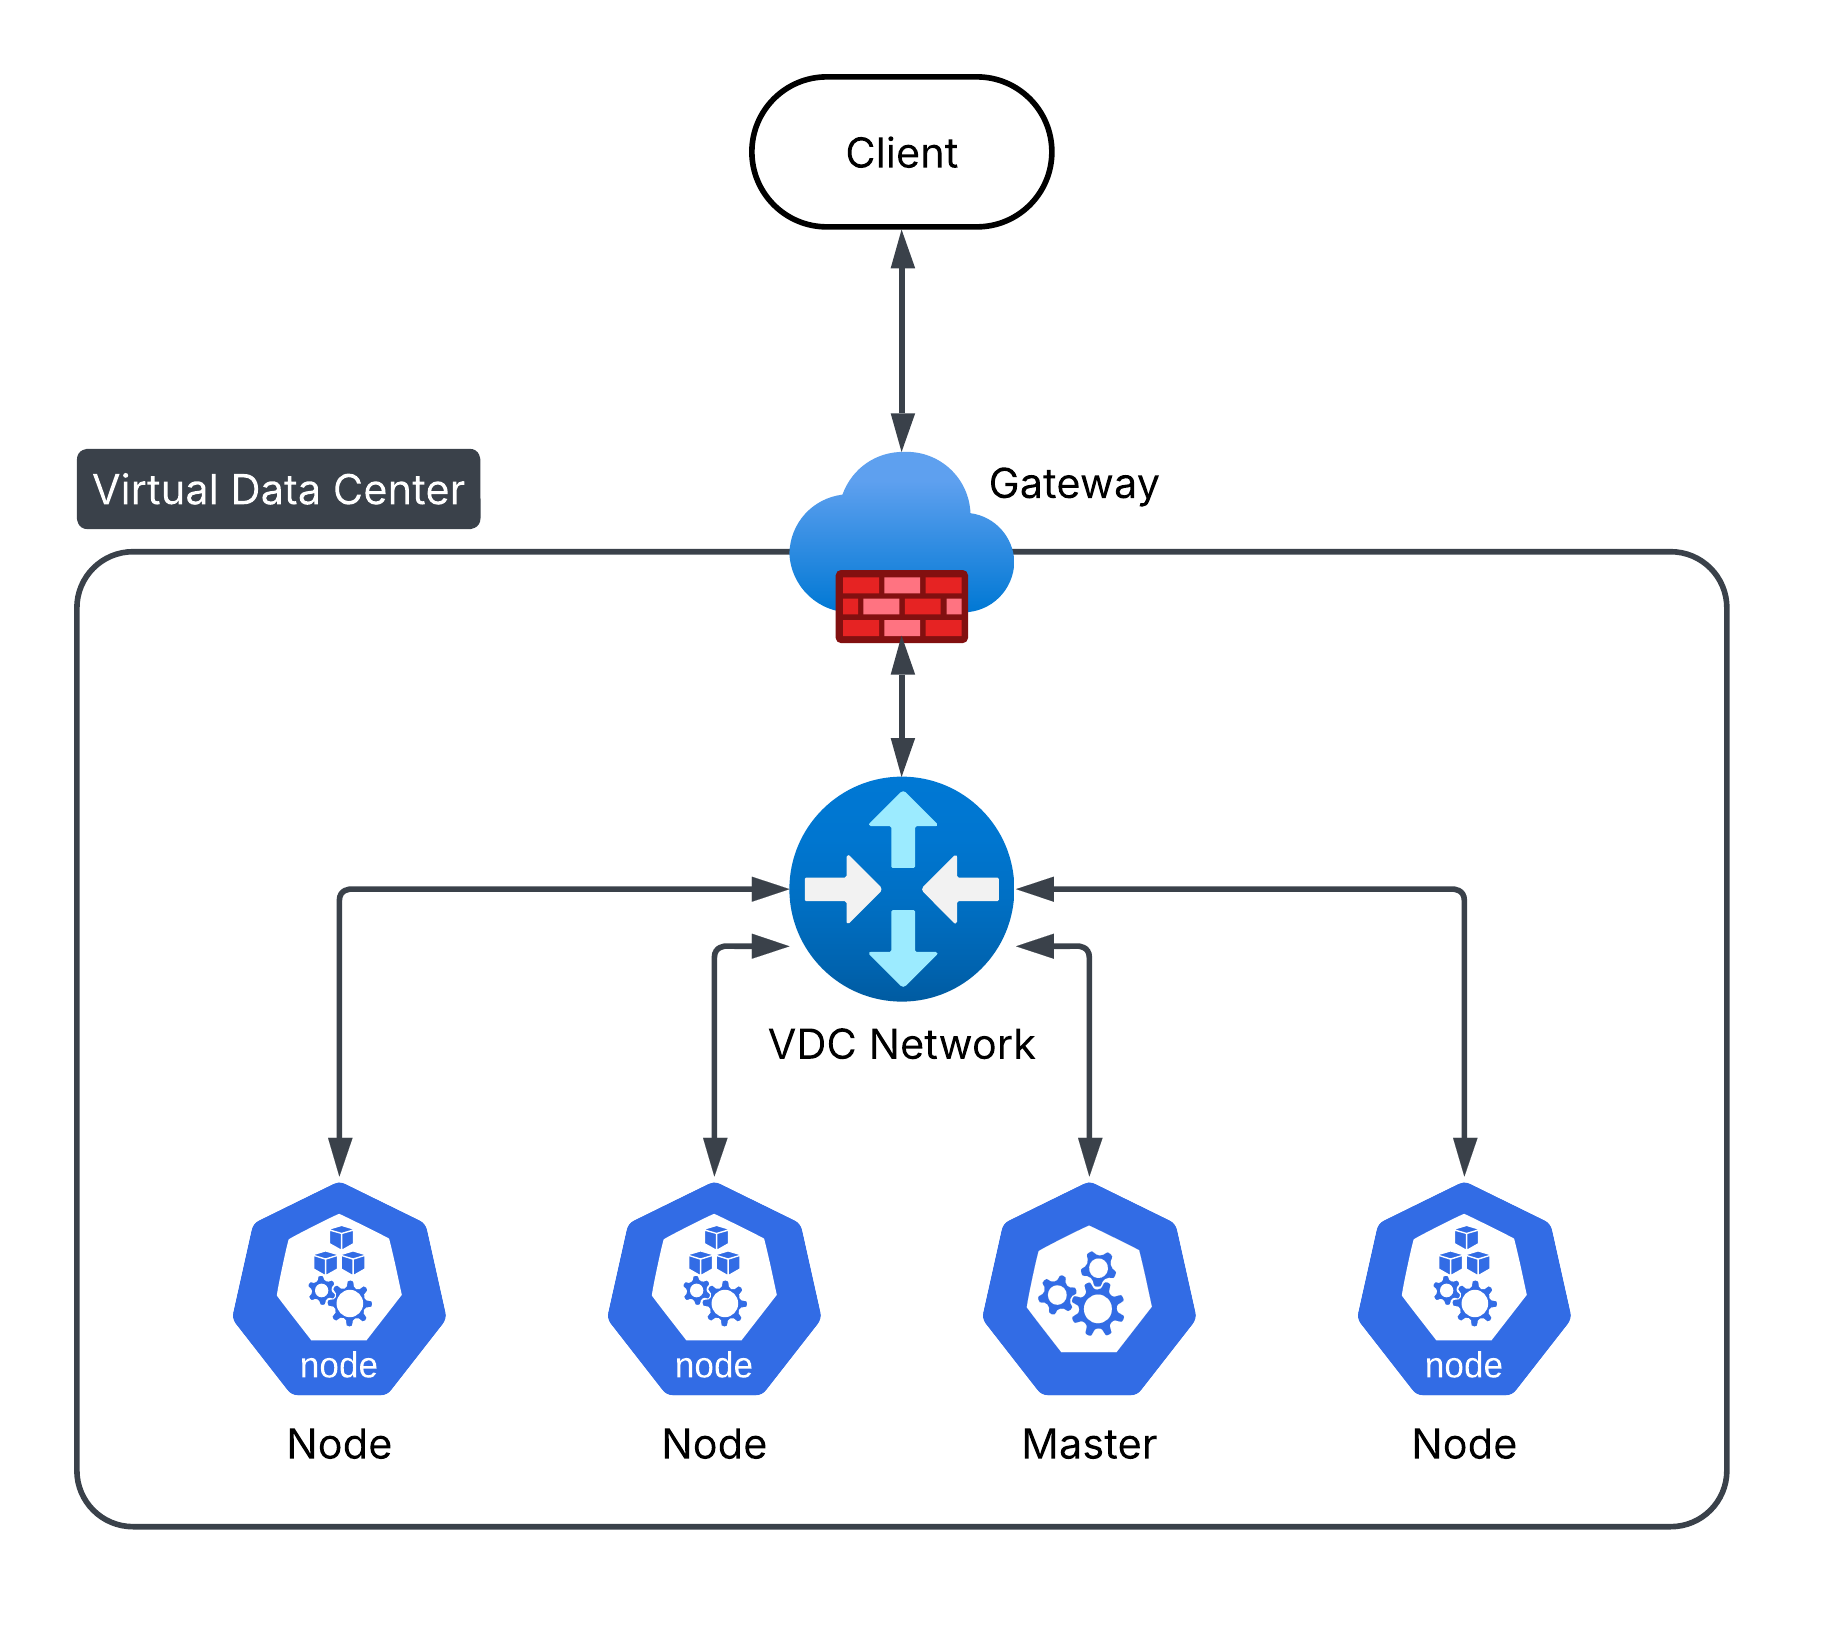
\includegraphics[width=0.5\textwidth]{figures/kube-vdc.png}
    \caption{Schema del cluster disposto su un VDC}
    \label{fig:kube-cluster}
\end{figure}
\section{Creazione del cluster}
La fase successiva è quella di integrazione dei nodi worker nel cluster. Questa operazione non è completamente automatizzata in quanto utilizzando
l'interfaccia grafica in congiunzione con \texttt{kubeadm} è necessario reperire un token di autenticazione che poi va inserito nei nodi worker.\\
Questo token viene generato dal nodo master e non è conosciuto a priori.\\
Ci sono diverse alternative per rendere questa fase il più automatica possible:
\begin{itemize}
    \item Utilizzo di API per automatizzare il processo di generazione e distribuzione dei token
    \item Implementazione di script che gestiscano automaticamente l'integrazione dei nodi worker
    \item Configurazione di sistemi di service discovery per l'auto-registrazione dei nodi
\end{itemize}
\subsection{Configurazione di un controller Ingress}
\label{sec:ingress}
Infine viene installato l'Ingress Controller, per questa implementazione è stato scelto \textit{NginX Ingress Controller}. Questo componente è solitamente
incluso nel servizio di Kubernetes dei cloud provider ma in questo caso è necessario comportarsi come se si stesse lavorando su macchine fisiche usando la 
versione \textbf{bare-metal} del controller.\\
Qui si possono scegliere due modalità di configurazione, anche in funzione delle operazioni che si vorranno svolgere nel cluster\cite{nginx-ingress-controller}:
\begin{itemize}
    \item \textbf{Utilizzo di MetalLB}: una soluzione unicamente software che permette l'utilizzo di load balancer anche in ambienti che non ne implementano.
        È comunque necessario che il cluster possa essere esposto all'esterno tramite un indirizzo IP pubblico. MetalLB si occupa di assegnare ad ogni servizio un
        indirizzo IP ed utilizza un nodo come punto di ingresso per il traffico esterno, successivamente annuncia tramite ARP che un servizio è raggiungibile tramite 
        quel nodo.\\
        Questo metodo non è implementabile perché il cluster è protetto da firewall mentre MetalLB ha bisogno di essere esposto completamente alla rete.
    \item \textbf{Esposizione tramite NodePort}: un metodo decisamente più semplice che consiste in impostare l'Ingress Controller in modalità NodePort.
        In questo modo il traffico esterno viene inviato ad una porta specifica di uno qualsiasi dei nodi del cluster, che poi lo inoltra al controller (che poi
        eseguirà il routing verso i servizi).\\
        In questo progetto è stata scelta questa modalità sia per motivi di semplicità nel testing sia perché il contesto non permette l'utilizzo di MetalLB.
\end{itemize} 
\chapter{Testing}
Per verificare il corretto funzionamento del cluster viene eseguita una semplica applicazione web stateless utilizzando NginX come server web. Il deployment consiste in due applicazioni
posizionate su più pod che servono due pagine web distinte, come per simulare l'erogazione di due servizi diversi.

I pod vengono racchiusi in un servizio che espone il suo endpoint al cluster; infine una risorsa Ingress espone il servizio all'esterno del cluster,
con le modalità menzionate alla \Cref{sec:ingress}, instradando il traffico verso i servizi in base al percorso richiesto.
\begin{figure}[!hbt]
    \centering
    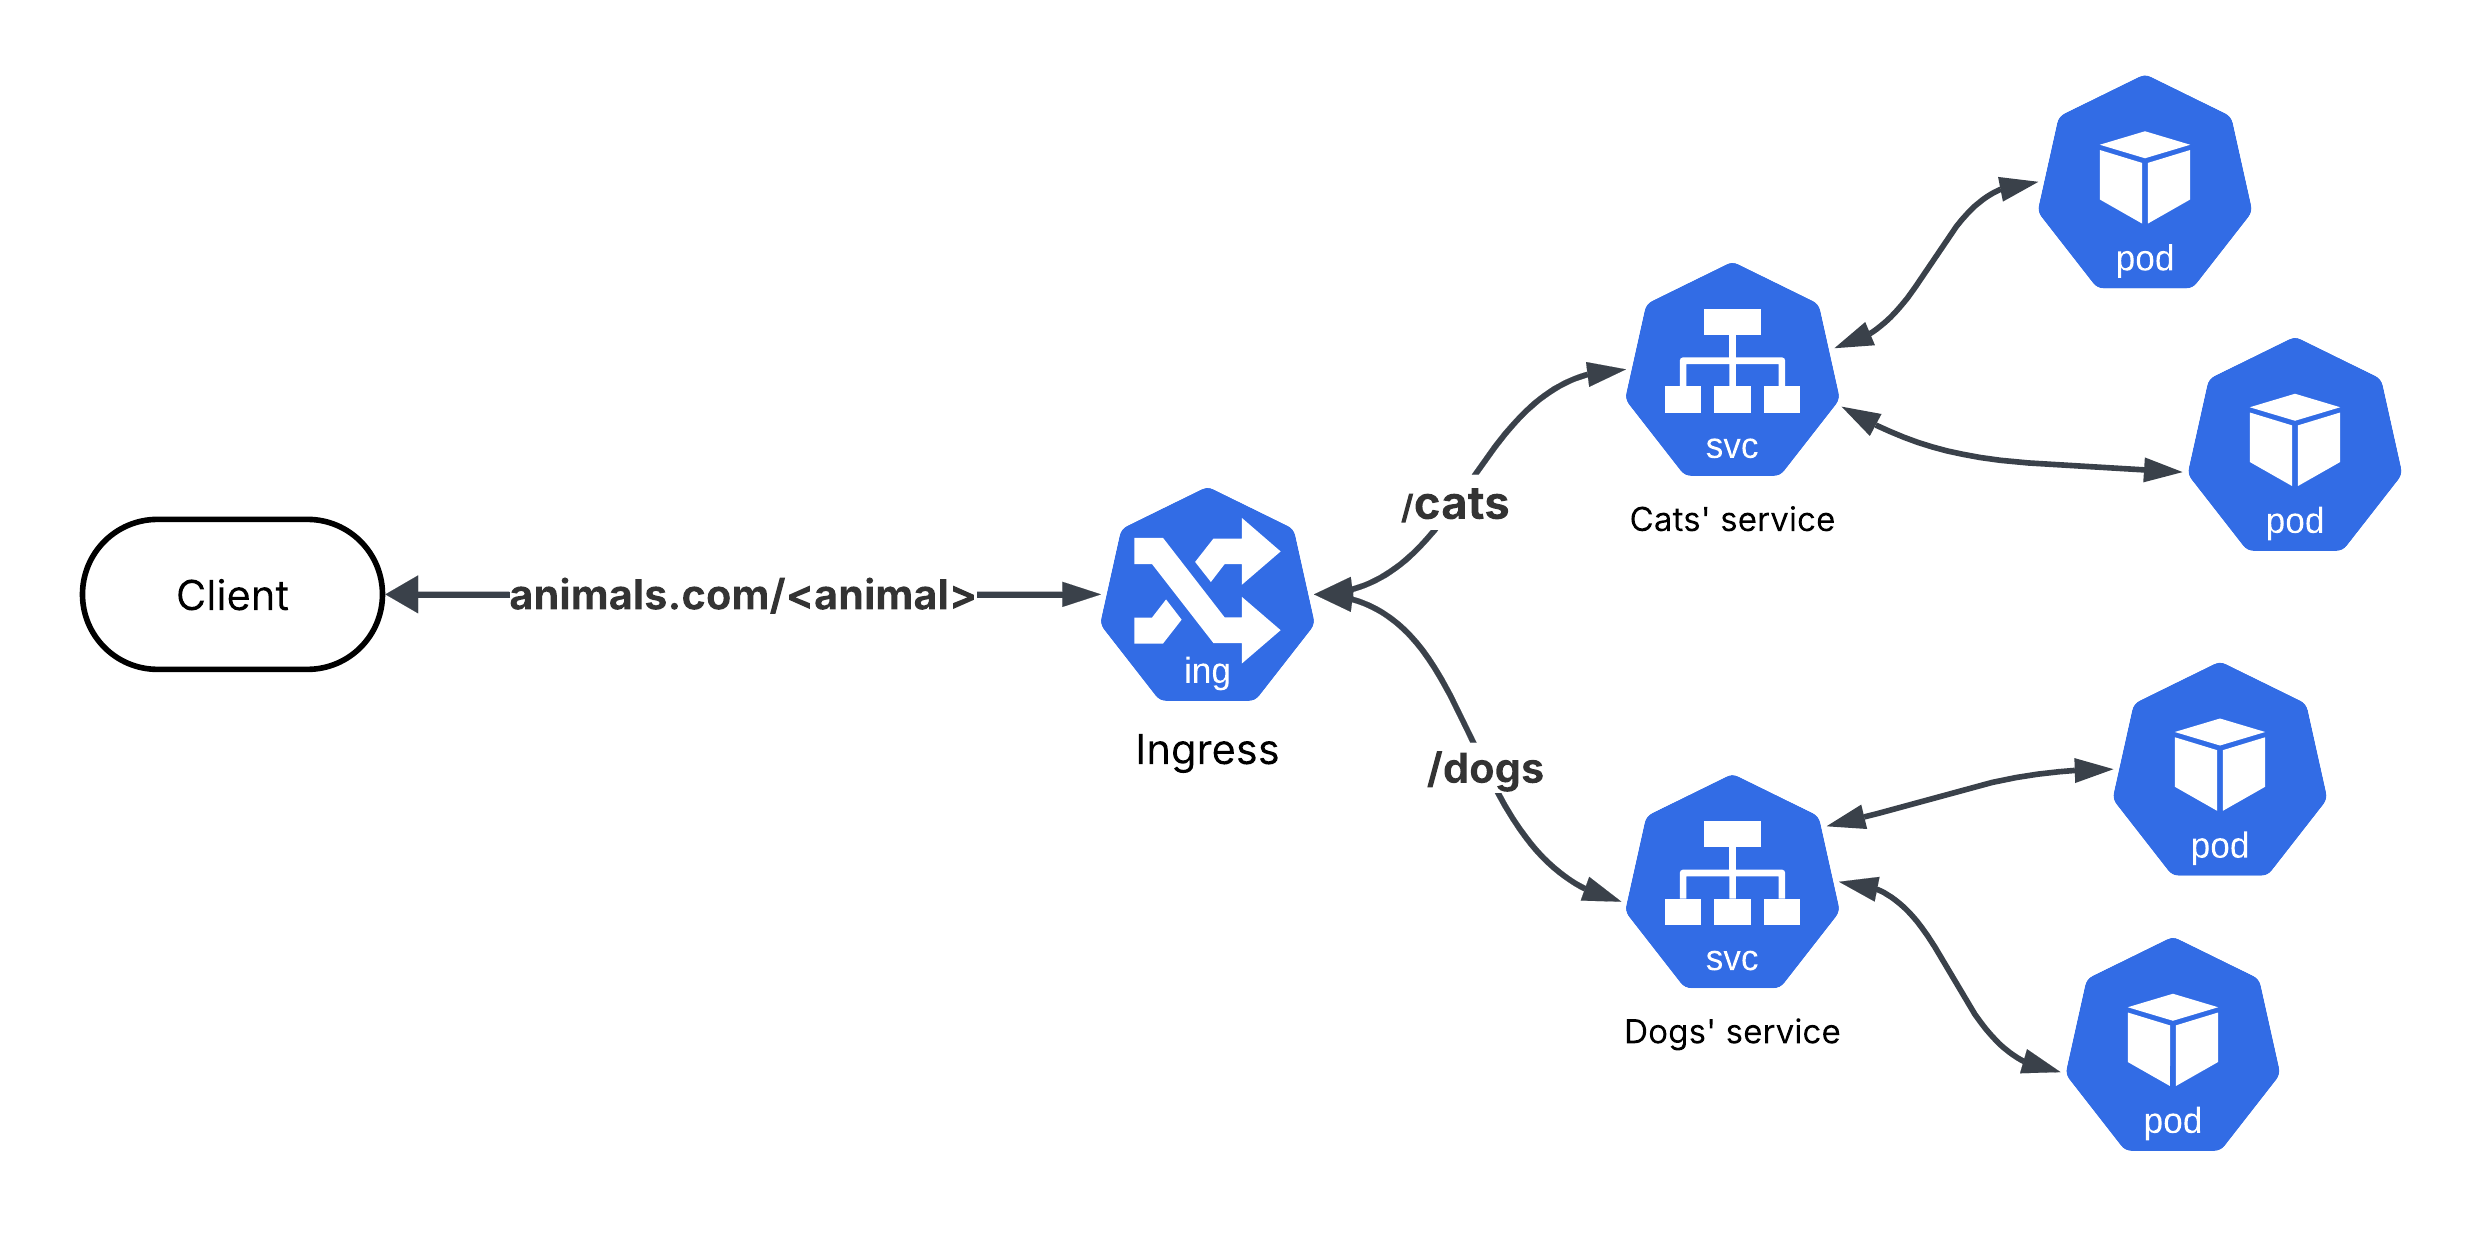
\includegraphics[width=0.9\textwidth]{figures/test-deployment.png}
    \caption{Schema del deployment di prova}
    \label{fig:test-deployment}
\end{figure}
\FloatBarrier
Il deployment viene applicato tramite i seguenti comandi:
\begin{lstlisting}
$ git clone https://github.com/bagarozzi/minikube-examples.git examples
$ kubectl apply -R -f examples/minikube/multiple-ingress/manifests
\end{lstlisting}
Prima di verificare il funzionamento bisogna recuperare la porta su cui è esposto, su ciascun nodo, l'Ingress Controller:
\begin{lstlisting}
$ kubectl get svc -n ingress-nginx                
\end{lstlisting}
Troveremo il numero di porta alla colonna \texttt{PORT(S)} della riga corrispondente al servizio \texttt{ingress-nginx-controller}.
% foto del comando o output codice?
Ora è possibile verificare il funzionamento in locale tramite \texttt{curl}. Il risultato sarà quello indicato al \Cref{lst:output-local}.
\begin{lstlisting}
$ curl -i -H "Host: www.animals.com" http://127.0.0.1:30900/cats
\end{lstlisting}
Successivamente si espone il cluster all'esterno aggiungendo una regola di port forwarding al firewall del VDC. Tramite questa si va a ridirezionare il traffico in ingresso verso
un nodo qualsiasi del cluster, sulla porta NodePort dell'Ingress Controller.
% foto della regola di port forwarding
Infine si verifica la disponiblità del servizio da un'altra macchina non collegata alla rete interna del VDC. 
\begin{lstlisting}
$ curl -i -H "Host: www.animals.com" http://gw-ingv-labdidattica.pp.ingv.it:17001/cats
\end{lstlisting}
Visto che il dominio che utilizzato (\texttt{www.animals.com}) non è inserito in nessun DNS non sarà possibile scrivere direttamente l'URL ma si dovrà aggiungere manualmente
l'indirizzo all'header della richiesta. In questo modo quando la richiesta viene inoltrata attraverso da Ingress questo saprà quale host si sta richiedendo,
senza questo accorgimento la richiesta arriverebbe al controller ma non verrebbe inoltrata a nessun servizio perché il campo header conterrebbe un altro dominio. 
\lstinputlisting[language=bash,label={lst:output-local}, caption=Output della richiesta cUrl]{listings/test-output.txt}
\chapter{Conclusione e lavori futuri}
%
% TODO: draft
%

%----------------------------------------------------------------------------------------
% BIBLIOGRAPHY
%----------------------------------------------------------------------------------------

\backmatter

\nocite{*} % Remove this as soon as you have the first citation

\bibliographystyle{alpha}
\bibliography{bibliography}

\begin{acknowledgements} % this is optional
Optional. Max 1 page.
\end{acknowledgements}

\end{document}
